\section{赤外線}
\subsection{赤外線ってなんだろう?}

\begin{figure}[H]
\centering
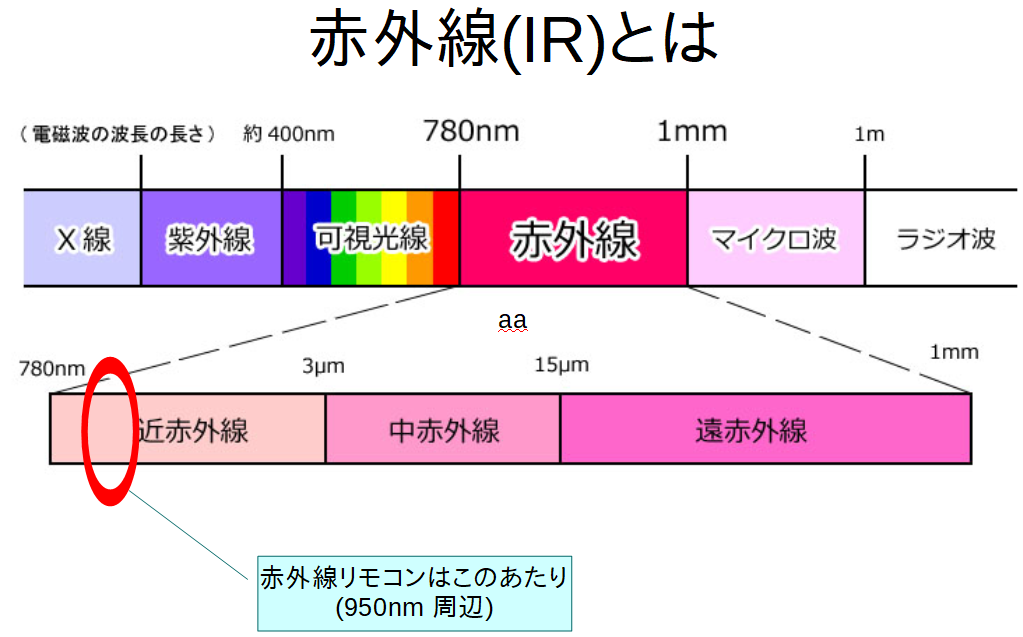
\includegraphics[scale=0.5]{images/chap05/text05-img036.png}
\caption{電磁波。出典: 家電 Watch \url{https://kaden.watch.impress.co.jp/cda/word/2008/11/21/3196.html} }

\end{figure}

物質や生物はそれぞれ電磁波を発しています。X線、紫外線、光、マイクロ波などは電磁波の一種です。電磁波は波であり、どれだけ振動しているかで種類をわけることができます。わたしたちは可視光線と呼ばれる光が目に入ることで、色などを目で感知することができます。マイクロ波は電子レンジに使われています。マイクロ波によって物質を振動させることで、物質の温度をあげています。\\

赤外線は人の目には見えません。けれどすべての物体が赤外線を発しています。特に温度の高いものは赤外線を強く発しています。Raspberry Piは発熱しながら動いています。Raspberry Piに触れなくても、手を近づけるだけで熱を感じるのは、赤外線がRaspberry Piから発せられていて、その赤外線を手で感知しているからです。\\

赤外線を使って信号を送ったり、受け取ったりすることもできます。例えば赤外線が送られているときは電気をつける、赤外線が送られていないときは電気を消すことができます。しかし送られているかどうかだけではつける、消すしかできません。ロボットのように歩く、止まる、右に曲がる、左に曲がるなど多くの動きを制御したいときは、信号を組み合わせて送ります。

\begin{figure}[H]
\centering
\includesvg[scale=0.6]{images/chap05/text05-img037.svg}
\caption{赤外線で信号を送る方法}
\label{ir}
\end{figure}

図\ref{ir}を見てみましょう。電球が点いているときは赤外線を送り、電球が消えていないときは赤外線を送っていないという意味です。例えば1/1000000秒の間隔で赤外線を送ります。つけたり消したりを組み合わせて、いろいろなパターンを作ることができます。そのパターンによって制御を決めています。送る、送らない、送らない、送らない、送る、送る、送らないと信号が来たときは”歩く”と制御します。
